
\documentclass[landscape,a0b,final]{a0poster}


\usepackage{epsfig}
\usepackage{multicol}
\usepackage{pstricks,pst-grad}
\usepackage{graphicx}
\usepackage{caption}
\usepackage{color}
\usepackage{amsmath}



%%%%%%%%%%%%%%%%%%%%%%%%%%%%%%%%%%%%%%%%%%%
% Definition of some variables and colors
%\renewcommand{\rho}{\varrho}
%\renewcommand{\phi}{\varphi}
\setlength{\columnsep}{2cm}
\setlength{\columnseprule}{0mm}
\setlength{\parindent}{0.0cm}




%%%%%%%%%%%%%%%%%%%%%%%%%%%%%%%%%%%%%%%%%%%%%%%%%%%%%%%%%%%%%%%%%%%%%%
%%% Begin of Document
%%%%%%%%%%%%%%%%%%%%%%%%%%%%%%%%%%%%%%%%%%%%%%%%%%%%%%%%%%%%%%%%%%%%%%

\begin{document}

\vspace*{1cm}


\newrgbcolor{lightblue}{0. 0. 0.80}
\newrgbcolor{white}{1. 1. 1.}
\newrgbcolor{whiteblue}{.80 .80 1.}

%%%%%%%%%%%%%%%%%%%%%
%%% Header
%%%%%%%%%%%%%%%%%%%%%
\begin{center}

%%% University seal
\hspace*{-9cm}
\begin{minipage}[c][9cm][c]{0.1\textwidth}
  \begin{center}
    \begin{tabular}{ccc}
    
\includegraphics[height=6cm,angle=0]{ucseal.pdf} &
    
\includegraphics[height=6cm,angle=0]{leeds.png} &
    
\includegraphics[height=6cm,angle=0]{maryland.png} 
    \end{tabular}
  \end{center}
\end{minipage}
%%% Title
\begin{minipage}[c][9cm][c]{0.78\textwidth}
  \begin{center}
    {\sc \Huge How is Mercury's dynamo powered?}\\[10mm]
    {\Large Grace Cox$^1$ Brent Delbridge$^2$, Jessica Irving$^3$, Hiroaki Matsui$^4$, William McDonough$^5$, Ian Rose$^2$, Anat Shahar$^6$, and Sean Wahl$^2$}\\[7.5mm]
    \emph{ $^1$University of Leeds, $^2$University of California at Berkeley, $^3$Princeton University, $^4$ University of California at Davis, $^5$University of Maryland, $^6$Carnegie Institute of Washington}\\[7.5mm]
    
\includegraphics[height=6cm,angle=0]{logo_cider.jpg} 
  \end{center}
\end{minipage}
\hspace*{-9cm}
%%% Department logo
\begin{minipage}[c][9cm][c]{0.1\textwidth}
  \begin{center}
    \begin{tabular}{ccc}
    
\includegraphics[height=6cm,angle=0]{princeton.png} &
    
\includegraphics[height=6cm,angle=0]{davis.png} &
    
\includegraphics[height=6cm,angle=0]{carnegie.png} 
    \end{tabular}
  \end{center}
\end{minipage}
\end{center}


\vspace*{1cm}


\begin{multicols}{3}

\section*{Introduction}

One of the more surprising findings of the MESSENGER spacecraft is the confirmation that the smallest terrestrial planet has an internally generated, dipolar magnetic field, which is likely driven by a combination of thermal and compositional buoyancy sources. 
This observation places constraints on the thermal and energetic state of Mercury’s large iron core and on mantle dynamics because dynamo operation is strongly dependent on the amount of heat extracted from the core by the mantle.
However, other observations point to several factors that should inhibit a present-day dynamo. 
These include physical constraints on a thin, possibly non-convecting mantle, as well as properties of liquid iron alloys that promote compositional stratification in the core.
We consider a range of self-consistent internal structures, core compositions and thermal evolution models that are also consistent with observational constraints, and assess the circumstances under which a dynamo is permitted to operate in Mercury’s core. 
We present the thermal evolution models, 1D parameterized convection models. 
We attempt to account for the large uncertainties on some parameters by considering various end member cases.
\\
\\
We examine the thermal and magnetic implications of a long-lived lateral temperature difference resulting from Mercury’s orbital resonance and how it may play a role in driving the planetary dynamo. 
To represent fluid dynamics and magnetic field generation inside Mercury’s core, a numerical dynamo model is performed by using the obtained heat flux maps.
Lastly, we also investigate the seismic observability of the different structural models of Mercury to determine the extent to which any future single-seismometer mission will be able to provide alternative insights into Mercury's internal dynamics.
\\
\\
This study was initiated at the 2014 CIDER summer program on the dynamics of planetary interiors.


\section*{Interior structure and core thermodynamics}

\begin{center}
\begin{tabular}{cc}
 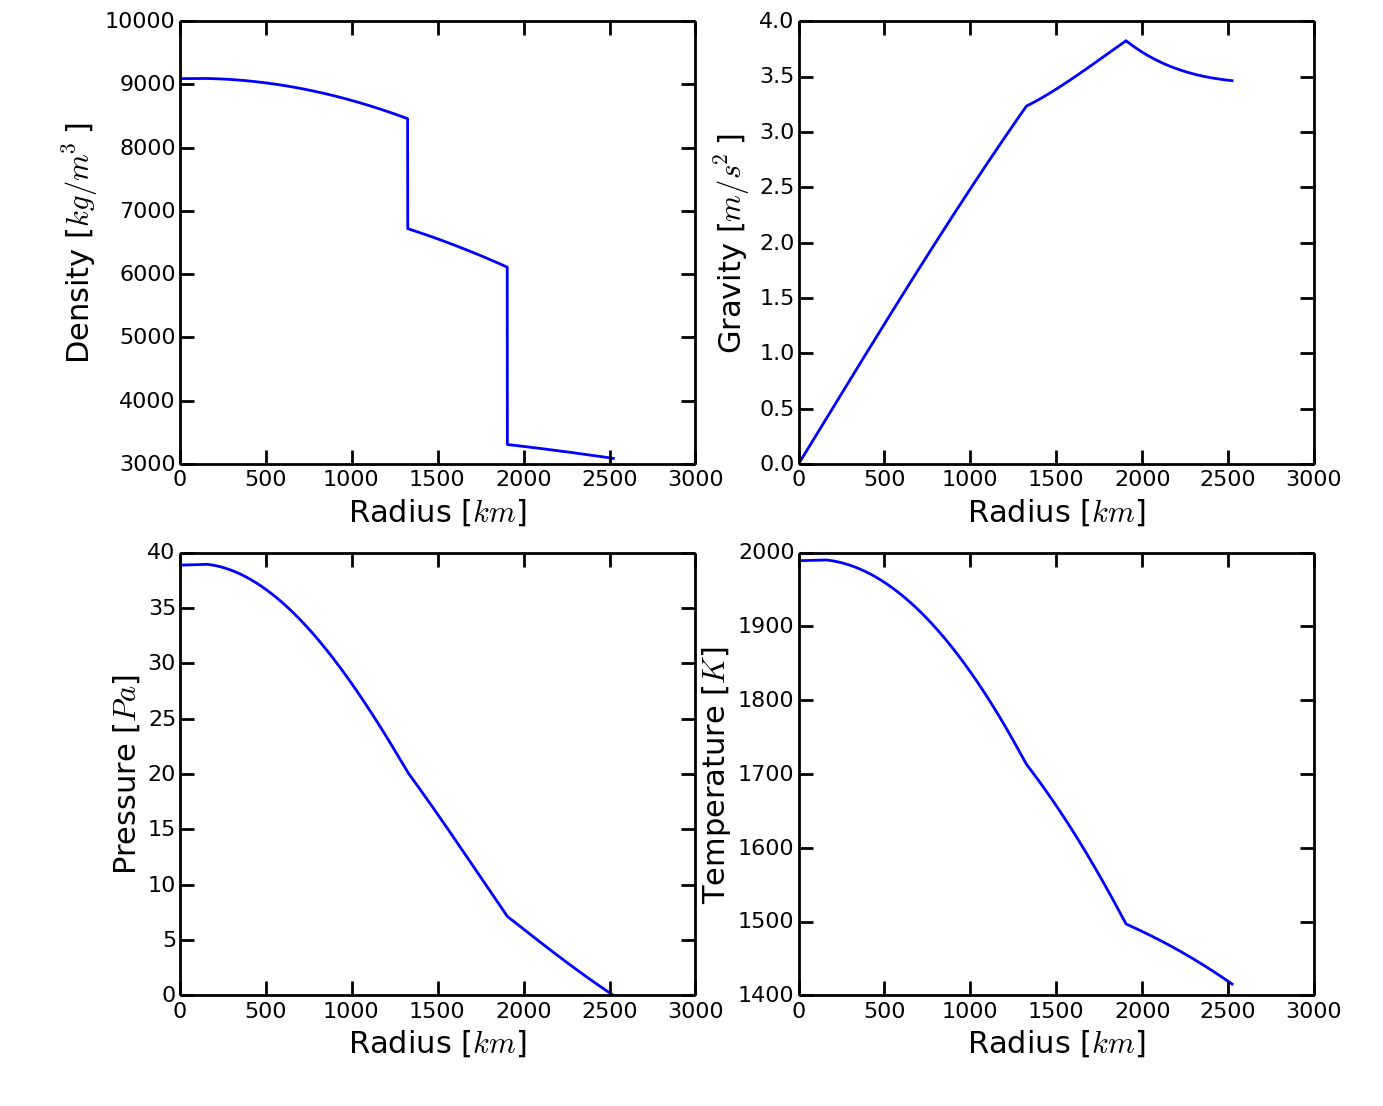
\includegraphics[width=0.15\textwidth]{profiles.png} &
 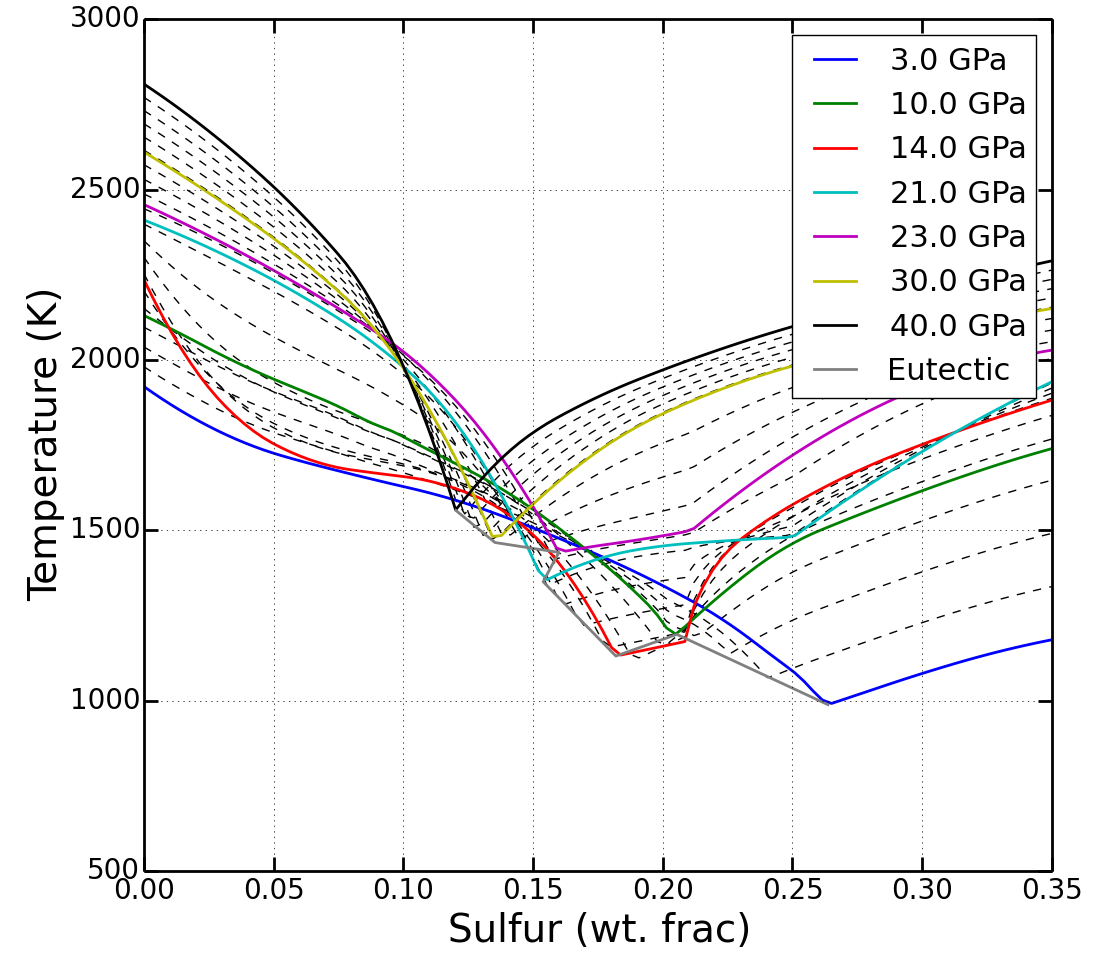
\includegraphics[width=0.15\textwidth]{Liquidus_model.png} \\
 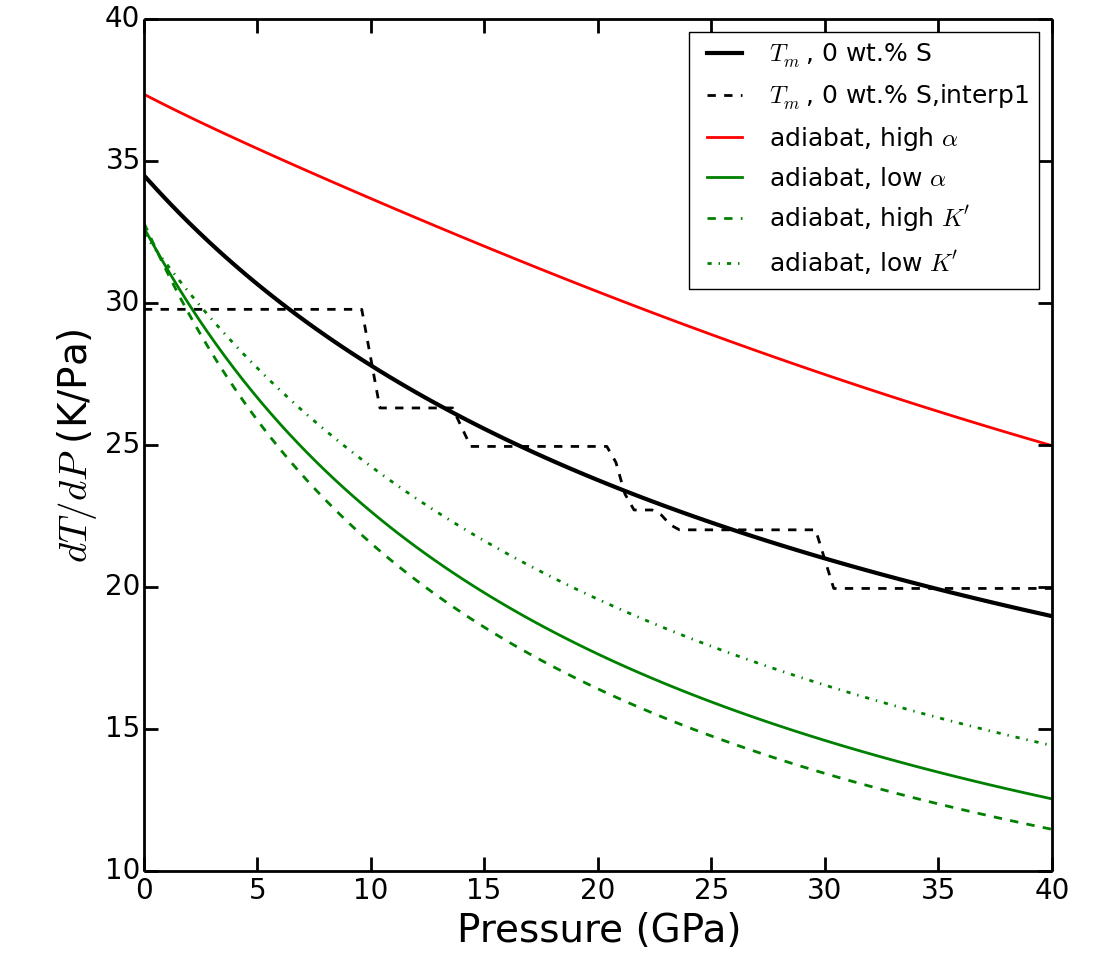
\includegraphics[width=0.15\textwidth]{clapeyron_1.png} &
 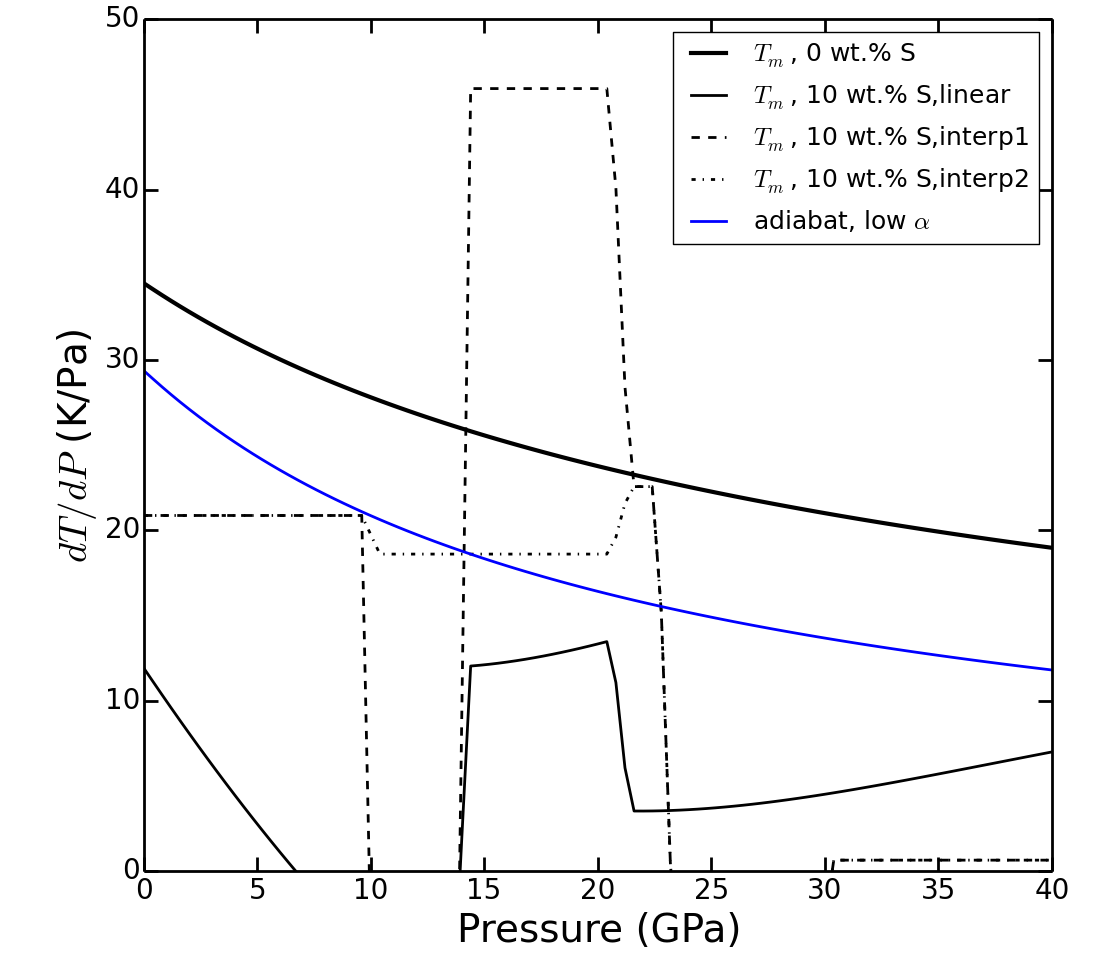
\includegraphics[width=0.15\textwidth]{clapeyron_2.png} \\
\end{tabular}
\captionof{figure}{ }
\label{interior_model}
\end{center}

\columnbreak

\section*{Parameterized convection and thermal evolution}



\section*{What if we had an InSight-style seismometer?}

\columnbreak

\section*{Dynamo simulation}

Mercury's unusual 3:2 spin-orbit resonance causes persistent temperature variations at the surface.  This boundary condition may create significant heat-flux variations at the CMB, especially if the mantle is not convecting.  Here we solve a simple conduction equation in the mercurian mantle to calculate an estimate of heat flux at the CMB.  This heat-flux variation is then used to inform the boundary conditions of a dynamo simulation using the \texttt{Calypso} code.

\begin{center}
\begin{tabular}{cc}
 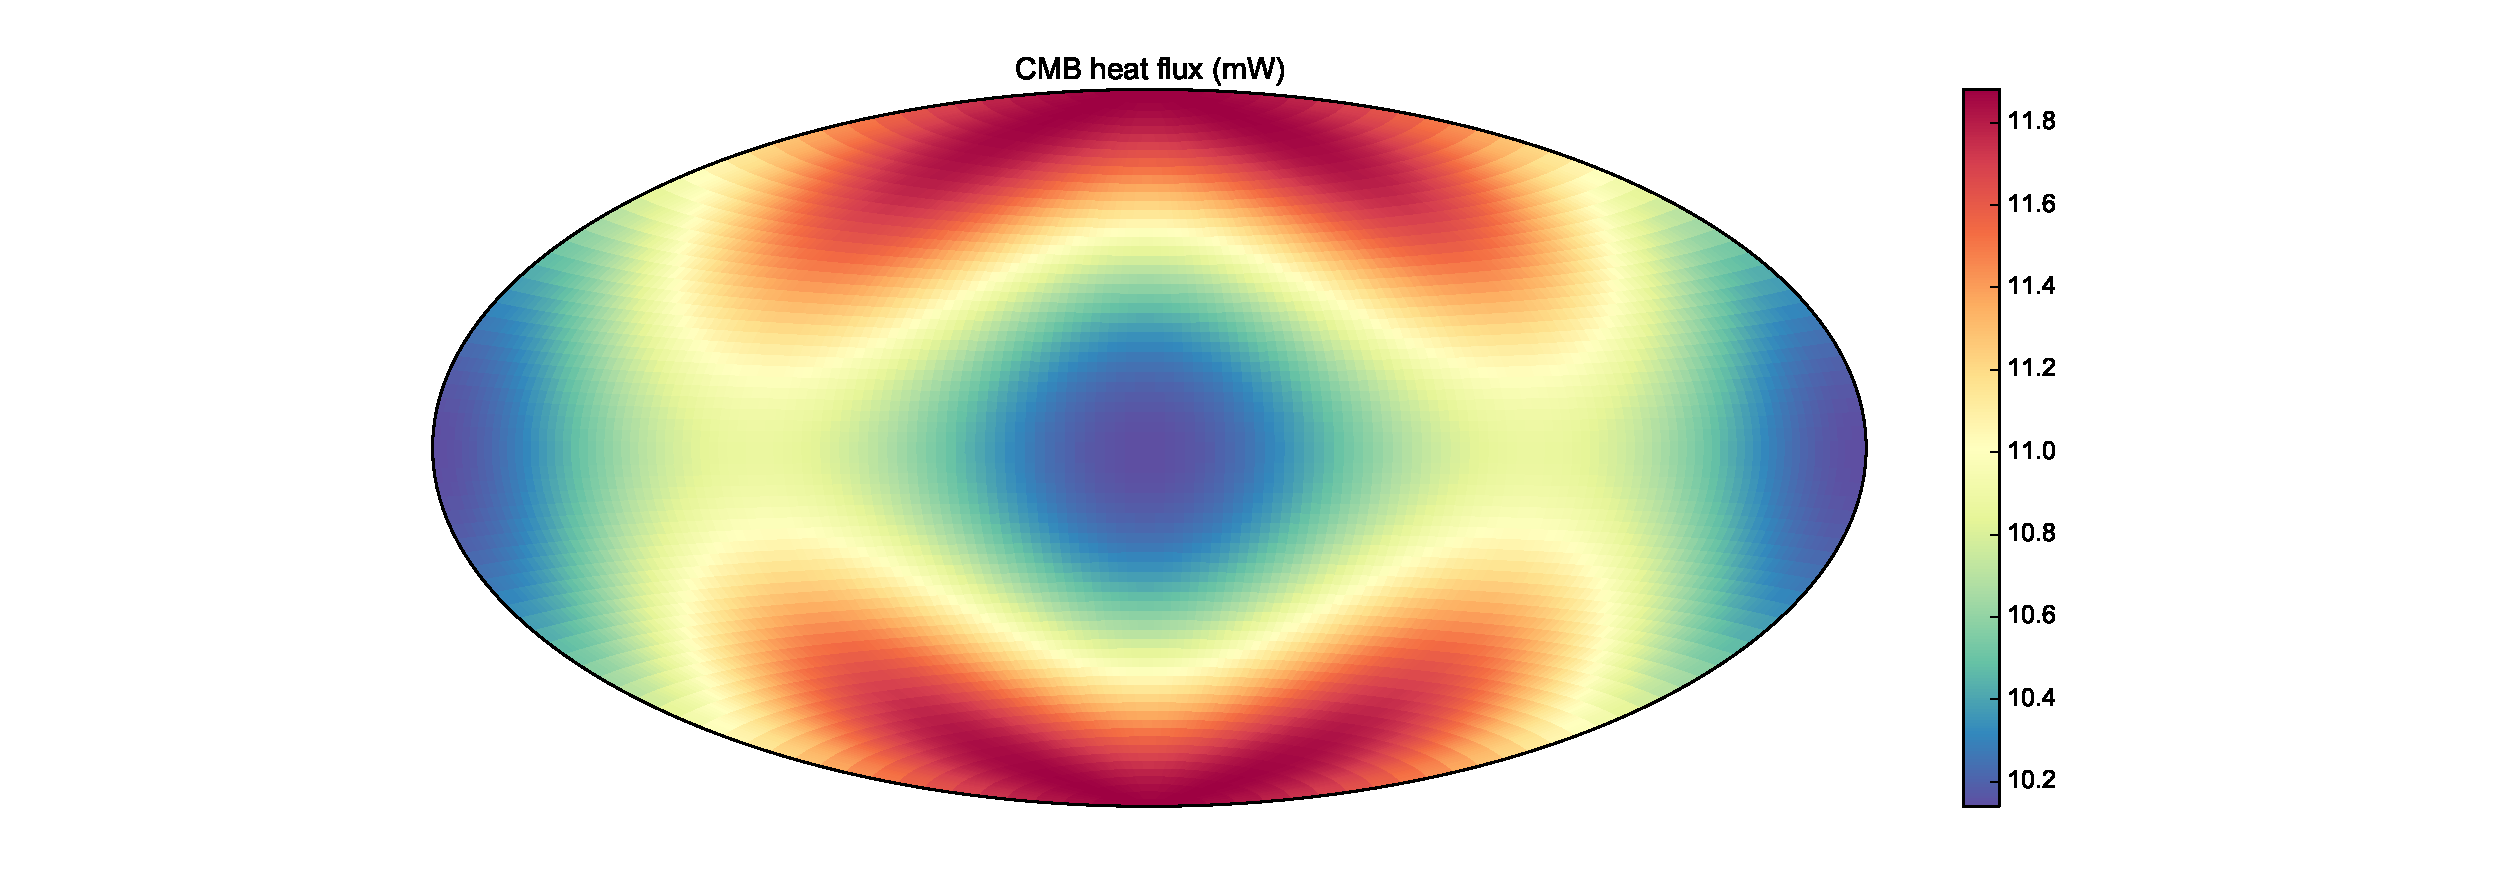
\includegraphics[width=0.18\textwidth]{CMB_flux.pdf} &
 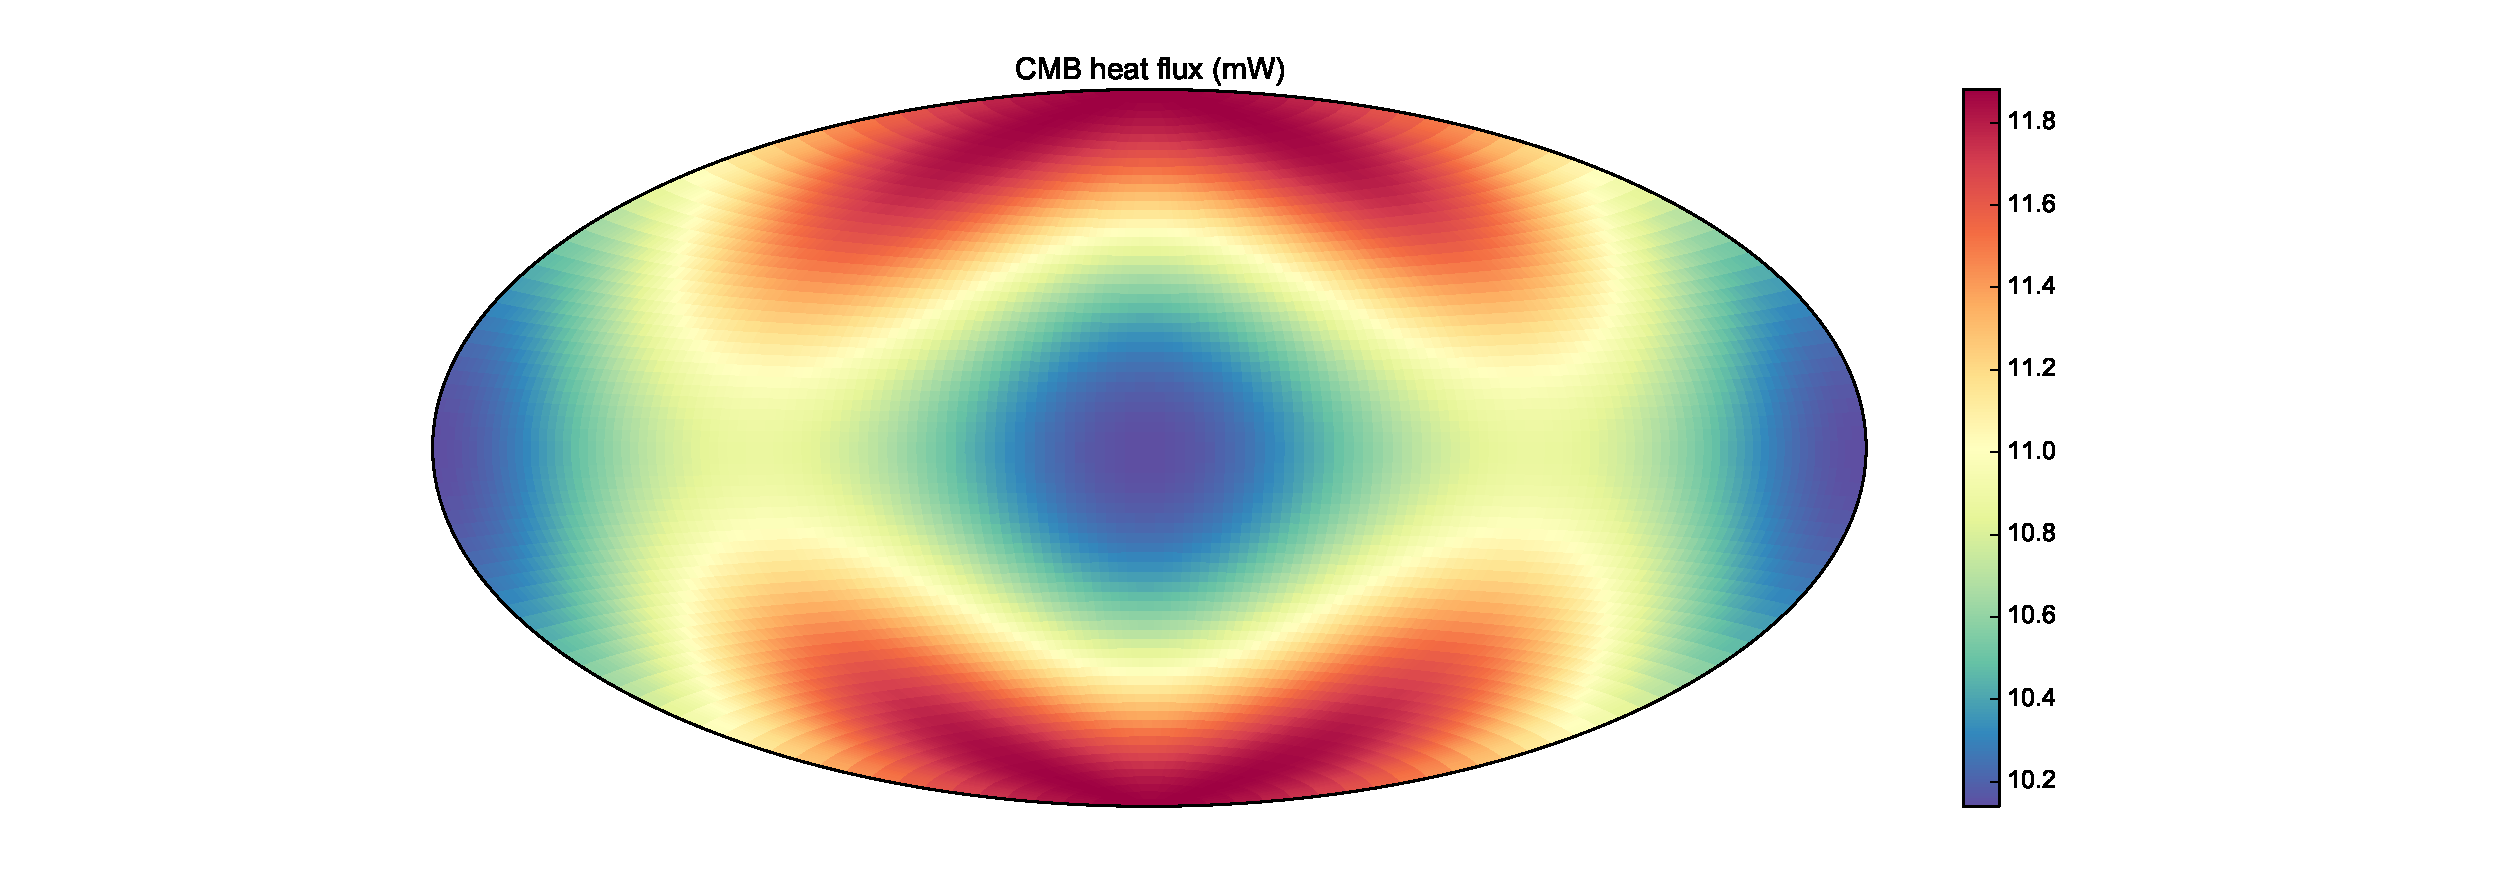
\includegraphics[width=0.15\textwidth]{CMB_flux.pdf} \\
 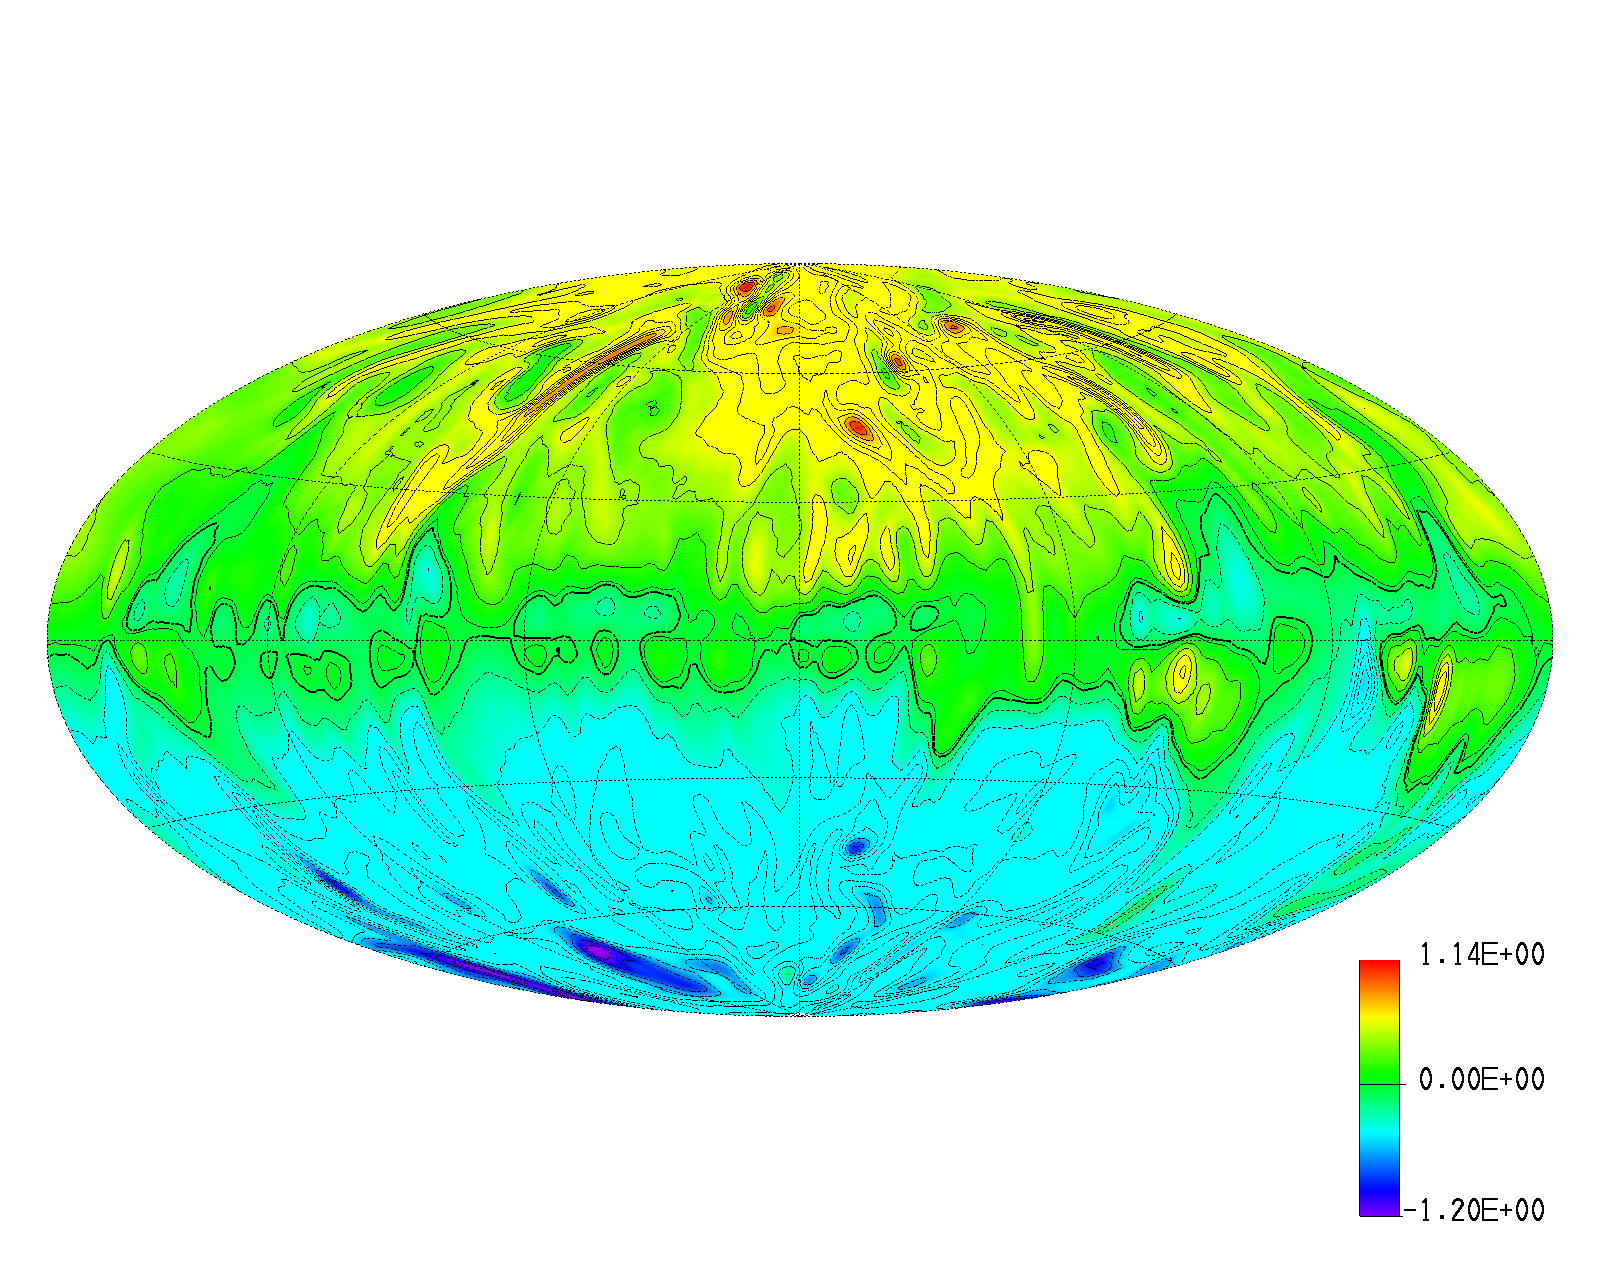
\includegraphics[width=0.12\textwidth]{br_cmb_x0.png} &
 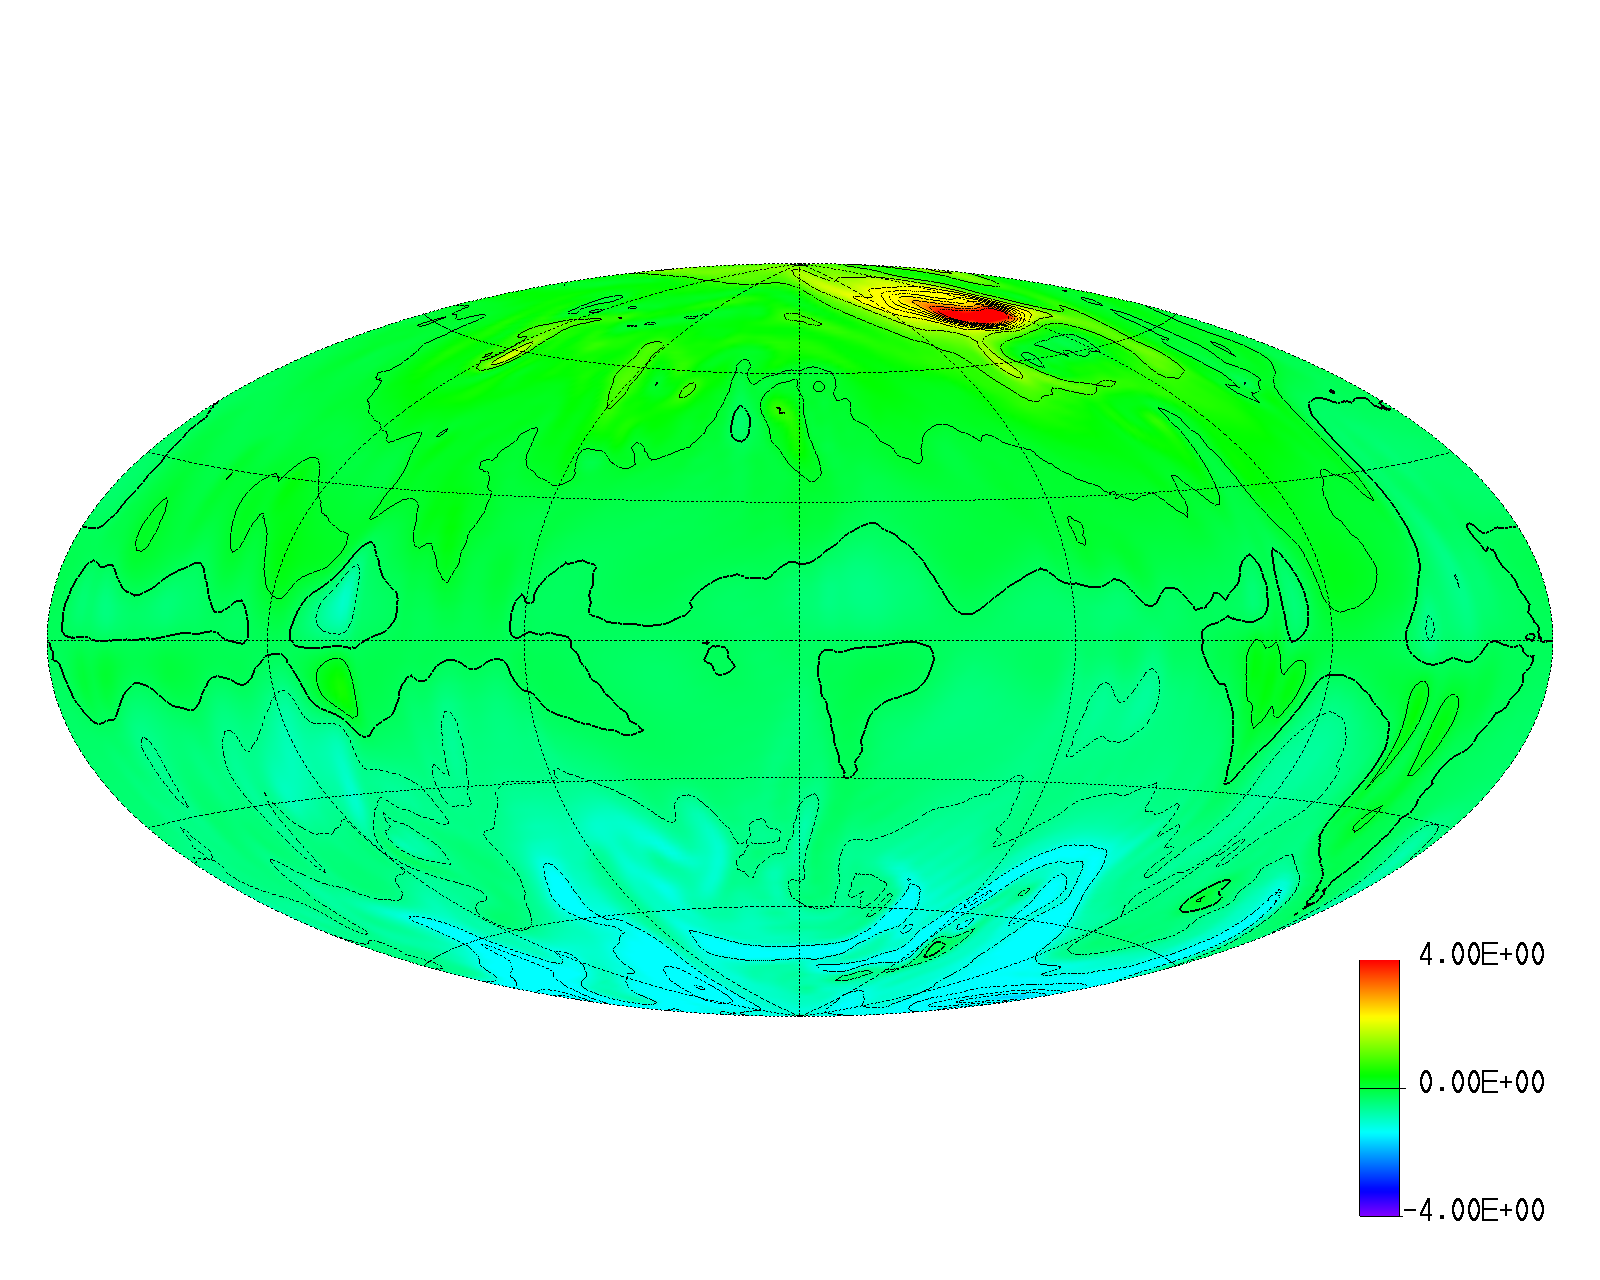
\includegraphics[width=0.12\textwidth]{br_cmb_x10.png}
\end{tabular}
\captionof{figure}{ }
\label{dynamo}
\end{center}


\fbox {\parbox[br]{0.30\textwidth}{ \large References \\ \small

} }


\end{multicols}


\end{document}

